\documentclass[reqno]{amsart}

\usepackage{amsmath,amssymb,amsthm}
\usepackage{fullpage}
\usepackage{tikz}
\usetikzlibrary{arrows.meta,shapes.geometric}

\newtheorem{theorem}{Theorem}[section]
\newtheorem{proposition}[theorem]{Proposition}
\newtheorem{lemma}[theorem]{Lemma}
\theoremstyle{remark}
\newtheorem{remark}[theorem]{Remark}

\numberwithin{equation}{section}

\newcommand{\Z}{\mathbb{Z}}

\begin{document}

\title{A dyadic graph construction for distinct subset sums}

\begin{abstract}
We construct, for every $n \geq 2$, a set of $n$ positive integers with distinct subset sums
and maximum less than $2^{n+1}/\log_2 n$.  The construction uses a dyadic directed graph with a small
determinant and an integer lattice excluding balanced relations.  Binary padding converts the
associated modular labels into positive integers.
\end{abstract}

\maketitle

\section{Introduction}

A finite set $A$ of positive integers is \emph{sum-distinct} if the map
$S \mapsto \sum_{a\in S}a$ is injective on the subsets of $A$, including the empty subset.  For
positive integers $n,N$, define
\[
f(n)=\min_{\substack{|A|=n\\ A\text{ sum-distinct}}}\max A,
\qquad
F(N)=\max_{\substack{A\subseteq\{1,\ldots,N\}\\ A\text{ sum-distinct}}}|A|.
\]
All logarithms are to be base 2.  Counting the $2^n$ subset sums in $[0,n\max A]$ gives
$f(n)\geq (2^n-1)/n$, whereas the powers of two give $f(n)\leq 2^{n-1}$.

\subsection{Background and history}

The problem appears in Erdős's 1956 survey, where he asks whether $F(N)=\log N+O(1)$ and
reports a second-moment argument with Moser giving $f(n)\gg 2^n/\sqrt n$ [4].  The proposed
estimate for $F$ is equivalent to a lower bound $f(n)\geq c2^n$ for some absolute constant
$c>0$.  On the construction side, Conway and Guy introduced a recursive sequence giving
$f(n)<2^{n-2}$ for sufficiently large $n$; Bohman proved that every set in this sequence is
sum-distinct [1].  Bohman's 1998 paper develops a broader construction giving
$f(n)<0.22002\mathbin{\cdot}2^n$ for sufficiently large $n$ [2].

Dubroff, Fox and Xu [3] proved the lower bound
\[
f(n)\geq\left(\sqrt{\frac{2}{\pi}}-o(1)\right)\frac{2^n}{\sqrt n},
\]
matching an earlier unpublished result of Elkies and Gleason.  They give proofs using normal
approximation and an isoperimetric inequality.

\subsection{Main result}

We prove the following quantitative improvement to the upper bound.

\begin{theorem}[Quantitative bound]
For every integer $n\geq 2$,
\[
f(n)<\frac{2^{n+1}}{\log n}.
\]
Consequently $f(n)/2^n\to 0$, so no positive absolute lower constant is possible.  For every
integer $N\geq 2^{16}$,
\[
F(N)\geq \left\lfloor\log N+\log\log\log N-1\right\rfloor.
\]
\end{theorem}

\subsection{Proof overview}

We first seek $r$ residues modulo $q$ whose equal-cardinality subset sums are distinct, with
$q$ substantially smaller than $2^r$.  We allow collisions between subsets of different sizes:
requiring all $2^r$ subset sums to be distinct modulo $q$ would force $q\geq 2^r$ by the
pigeonhole principle.  For integers $H\geq 1$, Proposition 2.1 supplies such sets with
$r\asymp 2^H$ and $q/2^r=O(1/H)$.

Section 2 explains why this weaker property suffices.  Choose representatives $0\leq c'_j<q$
and an integer $t\geq 0$.  Add the offset $b=(2^t+r)q$ to each representative, and adjoin the
$t$ binary multiples $q,2q,\ldots,2^{t-1}q$.  In an equality of integer subset sums, the offset
is too large to be cancelled unless both sides contain the same number of shifted labels.
Reduction modulo $q$ then determines those labels, and binary uniqueness determines the remaining
elements.  The resulting set $A$ has $r+t$ elements and
\[
\frac{\max A}{2^{r+t}}<\left(1+\frac{r+1}{2^t}\right)\frac{q}{2^r}.
\]
Taking $2^t$ of order $r^2$ makes the prefactor tend to one, while $r+t=r+O(\log r)$.  Thus
the saving $1/H$ in the modulus becomes a saving of order $1/\log n$ in the maximum.  Doubling
the set and adjoining 1 adds one element without changing the normalized maximum, allowing every
cardinality.

Section 3 constructs the modular sets from a directed graph on $r$ vertices, joining $2^H$
ordered stages to a tree of dyadic intervals.  Every cycle passes through an entry vertex $a$,
and every vertex has two outgoing edges except a root marker $d$, which has one.  If $E$ is the
adjacency matrix, put $M=2I_r-E$ and $q=\det M$.  Start a walk at $a$, choosing each outgoing
edge with probability $1/2$ and interpreting the missing probability at $d$ as death.  Stop at
death or the first return to $a$.  Then $q/2^r$ is the death probability.  The tree lets the walk
jump over dyadic blocks.  Let $u_h$ be the expected number of stages visited in a block of size
$2^h$, entered at its left endpoint, divided by $2^h$.  Splitting blocks into halves gives
\[
u_0=1,\qquad u_h=u_{h-1}-\frac{3}{16}u_{h-1}^2,\qquad
\frac{q}{2^r}=\frac{3}{8}u_H.
\]
The reciprocal $1/u_h$ grows linearly with $h$, giving the bound of order $1/H$.

The same graph rules out balanced ternary vectors in the row lattice $L=\Z^rM$, where a vector
is balanced if its coordinates sum to zero.  Suppose $p=zM$ has coordinates in $\{-1,0,1\}$
and is balanced.  The row sums force $z_d=0$.  Each positive coefficient of $z$ requires a
positive predecessor, and similarly for negative coefficients.  Each nonempty sign class
therefore contains a cycle; since every cycle contains $a$, both signs cannot occur.  After
reversing signs, a nonzero $z$ would contain a positive cycle.  Its transitions supply positive
dyadic markers covering the whole interval.  Two positive child markers force their parent
positive, so the covering forces $z_d>0$, a contradiction.

It remains to turn the lattice into a single modulus.  The determinant is odd, and the principal
minor at $a$ is $2^{r-1}$.  An adjugate column therefore defines a surjection $\Z^r\to\Z/q\Z$
with kernel exactly $L$.  The images of the coordinate vectors are the desired labels: a balanced
modular relation would lie in $L$, where the preceding argument excludes it.

\section{From modular sets to distinct subset sums}

\begin{proposition}[Modular set construction]
For integers $H\geq 1$, one can choose positive odd integers $q_H$ and sets
$C_H\subseteq\{0,\ldots,q_H-1\}$ of size $r_H=2^{H+2}-1$ such that, for any
$S,T\subseteq C_H$,
\[
|S|=|T|,\qquad
\sum_{c\in S}c\equiv\sum_{c\in T}c\pmod{q_H}
\quad\Longrightarrow\quad S=T.
\]
Moreover,
\[
0<\frac{q_H}{2^{r_H}}\leq\frac{2}{H+16/3},
\qquad
\frac{q_H}{2^{r_H}}\sim\frac{2}{H}\quad(H\to\infty).
\]
\end{proposition}

We deduce Theorem 1.1 from Proposition 2.1 using the following lemmas; the proof of the
proposition is deferred to Section 3.

\begin{lemma}[Binary padding]
Let $q\geq 1$ be an integer, and let $C\subseteq\{0,\ldots,q-1\}$ have size $r\geq 1$ and
distinct equal-cardinality subset sums modulo $q$.  For an integer $t\geq 0$, set
$b=(2^t+r)q$ and
\[
A=\{2^iq:0\leq i<t\}\cup\{b+c:c\in C\}.
\]
Then $A$ is sum-distinct, consists of $r+t$ positive integers, and
$\max A<(2^t+r+1)q$.
\end{lemma}

\begin{proof}
Write $C=\{c'_1,\ldots,c'_r\}$.  The shifted elements are distinct, positive, and larger than
every binary element, giving the cardinality and maximum.  A collision of subset sums would give
\[
\sum_{i=0}^{t-1}\alpha_i2^iq+b\sum_{j=1}^r\beta_j
+\sum_{j=1}^r\beta_jc'_j=0,
\qquad \alpha_i,\beta_j\in\{-1,0,1\}.
\tag{2.3}
\]
The first and third terms together have absolute value at most
$(2^t-1)q+r(q-1)<b$.  Since $\sum_j\beta_j$ is an integer, (2.3) forces this sum to be zero.
Reduction modulo $q$ shows that the positive and negative coordinates of $\beta$ select
equal-cardinality subsets of $C$ with the same sum modulo $q$.  By hypothesis these subsets
coincide; as they are disjoint, both are empty.  Thus $\beta=0$.  Then $\alpha=0$, because the
largest nonzero signed power of two exceeds the sum of all smaller powers.
\end{proof}

\begin{lemma}[Extension by parity]
If $A$ is a nonempty sum-distinct set of positive integers, then
$A^+=\{2a:a\in A\}\cup\{1\}$ is sum-distinct, $|A^+|=|A|+1$, and
$\max A^+=2\max A$.
\end{lemma}

\begin{proof}
Parity determines whether a subset contains 1; after removing it and dividing by 2,
sum-distinctness of $A$ determines the remaining subset.  The other assertions follow because all
doubled elements are distinct and at least 2.
\end{proof}

\begin{proof}[Proof of Theorem 1.1]
For each integer $H\geq 1$, take $q_H,C_H$ from Proposition 2.1, put
$r=r_H=2^{H+2}-1$ and $q=q_H$, and enumerate $C_H$ as $c'_1,\ldots,c'_r$.  Apply Lemma 2.2
with
\[
t=\left\lceil\log(r^2)\right\rceil=2H+4,
\qquad n_H=r+t=2^{H+2}+2^H+3.
\tag{2.4}
\]
Call the resulting set $A_H$ and its maximum $N_H$.  Since $2^t=(r+1)^2$, Proposition 2.1
and Lemma 2.2 give
\[
\frac{N_H}{2^{n_H}}
<\left(1+\frac{r+1}{2^t}\right)\frac{q}{2^r}
\leq\frac{2(1+2^{-H-2})}{H+16/3}.
\tag{2.5}
\]
For $n\geq 13=n_1$, choose the largest $H$ with $n_H\leq n$ and apply Lemma 2.3 exactly
$n-n_H$ times; the ratio of the maximum to $2^n$ is unchanged.  For $H\geq 1$,
\[
n<n_{H+1}<2^{H+4},
\qquad (H+4)(1+2^{-H-2})\leq H+16/3,
\]
where the second inequality follows from $(H+4)2^{-H-2}\leq 5/8<4/3$.  Thus (2.5) gives
$f(n)/2^n<2/(H+4)<2/\log n$.  For $2\leq n<13$, use the binary set, since $\log n<4$.
This proves the first bound and the claimed limit.

For the inverse bound, let $N\geq 2^{16}$, $L_0=\log N$, $T=\log\log L_0$, and
$n=\lfloor L_0+T-1\rfloor$.  Then $T\geq 2$, $n\geq L_0$, and
\[
2^{n+1}\leq 2^{L_0+T}=N\log L_0\leq N\log n.
\]
The first bound gives $f(n)<N$, so $F(N)\geq n$, as required.
\end{proof}

\begin{remark}[Asymptotics of the constructed sets]
The sets $A_H$ in the preceding proof satisfy $N_H/2^{n_H}\sim 2/H$: the ratio of
$N_H/2^{n_H}$ to $q/2^r$ lies between 1 and $1+2^{-H-2}$, and Proposition 2.1 gives
$q/2^r\sim 2/H$.  Since $\log n_H=H+2+o(1)$, their maxima are
$(2+o(1))2^{n_H}/\log n_H$.  The maximal-height parity extensions chosen above have maximum
$(2+o(1))2^n/\log n$, since $H=\log n+O(1)$; this describes the construction, not a matching
lower bound for $f$.  For $N\geq 2^{16}$, the uniform inverse bound gives
$F(N)>\log N+\log\log\log N-2$.  Along the original maxima it sharpens to
$F(N_H)\geq n_H=\log N_H+\log\log\log N_H-1+o(1)$, because both
$\log\log\log N_H$ and $n_H-\log N_H+1$ equal $\log H+o(1)$.
\end{remark}

\section{Construction of the modular set}

It remains to prove Proposition 2.1.  We construct the matrix $M$ from a dyadic graph, estimate
its determinant, exclude balanced ternary vectors from its row lattice, and identify the resulting
quotient with a cyclic group.

\subsection{The dyadic graph}

Throughout Section 3, fix an integer $H\geq 1$, and put $m=2^H$ and $r=4m-1$.  Let $\mathcal D$
consist of the intervals $[t2^h,(t+1)2^h)$ for integers $0\leq h\leq H$ and
$0\leq t<m/2^h$.  Write $e(I)$ for the right endpoint.  For $I\neq[0,m)$, let
$\operatorname{par}(I)$ be the dyadic interval of twice its length containing it.  The vertices
are
\[
V=\{x_i,y_i:0\leq i<m\}\cup\{w_I:I\in\mathcal D\}.
\]
Set $a=x_0$, $d=w_{[0,m)}$, and use $x_m=x_0$ as an alias, not a new vertex.  The edges are
\begin{equation}
\begin{aligned}
x_i&\longrightarrow y_i,\ w_{[i,i+1)},
&y_i&\longrightarrow x_{i+1},\ w_{[i,i+1)} &&(0\leq i<m),\\
w_I&\longrightarrow x_{e(I)},\ w_{\operatorname{par}(I)},
&d&\longrightarrow a &&(I\neq[0,m)).
\end{aligned}
\tag{3.1}
\end{equation}
Figure 1 shows the construction for $H=2$.  Let $E$ be the adjacency matrix with outgoing edges
in rows, and define $M=2I_r-E$, $q=\det M$, and $\bar a=V\setminus\{a\}$.

\begin{figure}[ht]
\centering
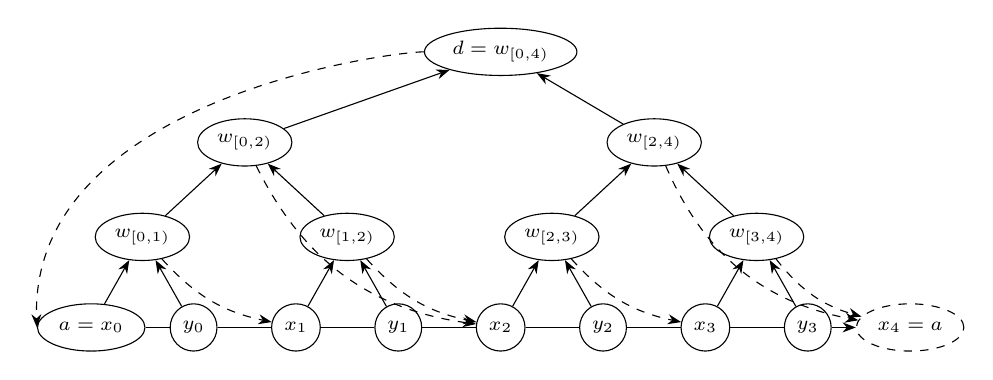
\begin{tikzpicture}[
  >=Stealth,
  every node/.style={font=\scriptsize},
  vertex/.style={draw, ellipse, inner sep=2pt, minimum height=6mm},
  marker/.style={draw, ellipse, inner sep=2pt, minimum height=6mm}
]
  \node[vertex] (a) at (0,0) {$a=x_0$};
  \node[vertex] (y0) at (1.3,0) {$y_0$};
  \node[vertex] (x1) at (2.6,0) {$x_1$};
  \node[vertex] (y1) at (3.9,0) {$y_1$};
  \node[vertex] (x2) at (5.2,0) {$x_2$};
  \node[vertex] (y2) at (6.5,0) {$y_2$};
  \node[vertex] (x3) at (7.8,0) {$x_3$};
  \node[vertex] (y3) at (9.1,0) {$y_3$};
  \node[vertex,dashed] (x4) at (10.4,0) {$x_4=a$};

  \node[marker] (w01) at (0.65,1.15) {$w_{[0,1)}$};
  \node[marker] (w12) at (3.25,1.15) {$w_{[1,2)}$};
  \node[marker] (w23) at (5.85,1.15) {$w_{[2,3)}$};
  \node[marker] (w34) at (8.45,1.15) {$w_{[3,4)}$};
  \node[marker] (w02) at (1.95,2.35) {$w_{[0,2)}$};
  \node[marker] (w24) at (7.15,2.35) {$w_{[2,4)}$};
  \node[marker] (d) at (5.2,3.5) {$d=w_{[0,4)}$};

  \draw[->] (a)--(y0)--(x1)--(y1)--(x2)--(y2)--(x3)--(y3)--(x4);
  \draw[->] (a) -- (w01);
  \draw[->] (y0) -- (w01);
  \draw[->] (x1) -- (w12);
  \draw[->] (y1) -- (w12);
  \draw[->] (x2) -- (w23);
  \draw[->] (y2) -- (w23);
  \draw[->] (x3) -- (w34);
  \draw[->] (y3) -- (w34);
  \draw[->] (w01) -- (w02);
  \draw[->] (w12) -- (w02);
  \draw[->] (w23) -- (w24);
  \draw[->] (w34) -- (w24);
  \draw[->] (w02) -- (d);
  \draw[->] (w24) -- (d);

  \draw[->,dashed] (w01) to[bend right=18] (x1);
  \draw[->,dashed] (w12) to[bend right=18] (x2);
  \draw[->,dashed] (w23) to[bend right=18] (x3);
  \draw[->,dashed] (w34) to[bend right=18] (x4);
  \draw[->,dashed] (w02) to[bend right=28] (x2);
  \draw[->,dashed] (w24) to[bend right=28] (x4);
  \draw[->,dashed] (d.west) .. controls (3.8,3.5) and (-0.8,2.9) .. (a.west);
\end{tikzpicture}
\caption{The graph for $H=2$ ($m=4$, $r=15$). Solid arrows are stage and parent edges;
dashed arrows are marker exits. The right-hand $x_4=a$ repeats $x_0$, not a new vertex.}
\end{figure}

\begin{lemma}[Graph structure]
The graph has $r$ vertices and is acyclic after deletion of $a$.  Every row of $M$ has sum zero
except row $d$, which has sum one.  Moreover,
\[
\det M_{\bar a,\bar a}=2^{r-1}.
\]
\end{lemma}

\begin{proof}
There are $2m$ stage vertices and $2m-1$ markers.  After deleting $a$, order markers by right
endpoint, shorter first at a tie, and place $x_i,y_i$ after markers ending at $i$ and before those
ending at $i+1$.  Every edge points forward, so $E_{\bar a,\bar a}$ is strictly upper triangular.
This proves (3.2); the row sums follow from (3.1).
\end{proof}

\subsection{The determinant estimate}

The next proposition gives the quantitative modulus bound in Proposition 2.1.

\begin{proposition}[A small positive determinant]
Define $u_0=1$ and $u_h=u_{h-1}-(3/16)u_{h-1}^2$ for $h\geq 1$.  Then
\[
0<\frac{q}{2^r}=\frac{3}{8}u_H\leq\frac{2}{H+16/3},
\qquad 0<u_H\leq\frac{1}{1+3H/16}.
\]
As $H\to\infty$, one also has $u_H\sim 16/(3H)$ and $q/2^r\sim 2/H$.
\end{proposition}

\begin{proof}
Put $B=E/2$.  Interpret $B$ as a transition rule that chooses each outgoing edge with
probability $1/2$, with the missing probability $1/2$ at $d$ meaning death.  Start at $a$ and
stop at the first return to $a$ or at death.  By Lemma 3.1, the submatrix
$B_{\bar a,\bar a}$ is nilpotent.  Hence
$\det(\operatorname{Id}-B_{\bar a,\bar a})=1$ and its inverse is a finite geometric series.
The block determinant formula, using $B_{a,a}=0$, yields
\[
\frac{q}{2^r}=1-R,
\qquad
R=B_{a,\bar a}(\operatorname{Id}-B_{\bar a,\bar a})^{-1}B_{\bar a,a}.
\tag{3.4}
\]
The power expansion identifies $R$ with the return probability.  Every excursion is finite, and
death can occur only at $d$, where return and death are equally likely.  It follows that
\[
\frac{q}{2^r}=\frac{1}{2}\mathbb P_a(\text{hit $d$ before returning to $a$})>0.
\tag{3.5}
\]
The inequality is strict because the path from $a$ to $w_{[0,1)}$ and then through its successive
parents reaches $d$ with positive probability.

Record the indices of visits to $x_i$ until a hit to $d$ or a return.  These indices increase
strictly; a return is an exit at index $m$, not another visit to index zero.  At a visited stage,
the walk takes $x_i\to y_i\to x_{i+1}$ with probability $1/4$ and reaches the leaf marker with
probability $3/4$.  At each proper marker it exits to the right endpoint or ascends to the parent,
each with probability $1/2$.  Thus the height $k$ of the next transition has the following
conditional law, independent of the past:
\[
\mathbb P(k=0)=\frac{5}{8},\qquad
\mathbb P(k=j)=\frac{3}{4}2^{-j-1}\quad(1\leq j<H),\qquad
\mathbb P(k=H)=\alpha_H=\frac{3}{4}2^{-H}.
\tag{3.6}
\]
For $k<H$, the next index is
$e_k(i)=\left(\left\lfloor i/2^k\right\rfloor+1\right)2^k$; height $H$ means a hit to $d$.
In particular $s_h:=\mathbb P(k\geq h)=(3/4)2^{-h}$ for $1\leq h\leq H$.

For $0\leq h\leq H$, let $b_h$ be the expected number of stage visits in a dyadic block of
size $2^h$ entered at its left endpoint, before leaving that block.  This expectation depends
only on $h$: heights below $h$ have the same relative endpoints in every aligned block, and all
larger heights leave it.  We claim
\[
b_0=1,\qquad b_h=2b_{h-1}-s_hb_{h-1}^2\quad(1\leq h\leq H).
\tag{3.7}
\]
Indeed, the expected visits in the left half are $b_{h-1}$.  A height at least $h$ at any of them
skips the right half.  These skip events are disjoint, since each exits the block, so their
probability is $s_hb_{h-1}$.  Otherwise the first index outside the left half is the midpoint,
since every smaller-height endpoint is at most the midpoint.  Conditional on entering the right
half, its expected visits are again $b_{h-1}$ by the transition law.  This gives
$b_h=b_{h-1}+(1-s_hb_{h-1})b_{h-1}$, proving (3.7).

Consequently $b_h/2^h$ satisfies the defining recurrence for $u_h$.  On the full block, a hit to
$d$ has conditional probability $\alpha_H$ at each visited stage.  These events are disjoint, so
the hit probability is $\alpha_Hb_H$.  Equation (3.5) now gives $q/2^r=(3/8)u_H$.  Induction
in the recurrence gives $0<u_h\leq 1$, and
\[
\frac{1}{u_h}-\frac{1}{u_{h-1}}
=\frac{3/16}{1-(3/16)u_{h-1}}\geq\frac{3}{16}.
\tag{3.8}
\]
Summing proves (3.3).  It also gives $u_H\to 0$, so the reciprocal increments in (3.8) tend to
$3/16$.  Averaging the increments yields $(1/u_H)/H\to 3/16$, which proves both asymptotic
equivalences.
\end{proof}

\subsection{Excluding balanced lattice relations}

The determinant estimate controls the size of the modulus.  We next prove the property that will
separate equal-cardinality subset sums.  Write $L=\Z^rM$ for the integer row lattice of $M$.

\begin{lemma}[Balanced ternary avoidance]
If $p\in L$, $p_j\in\{-1,0,1\}$ for every $j\in V$, and $\sum_jp_j=0$, then $p=0$.
\end{lemma}

\begin{proof}
Write $p=zM$ with $z\in\Z^r$.  By Lemma 3.1,
$z_d=\sum_jp_j=0$.  Every vertex with $z_j>0$ has a positive predecessor, since otherwise
\[
p_j=2z_j-\sum_{i\to j}z_i\geq 2.
\]
The analogous assertion holds for negative vertices.  Following predecessors in a nonempty sign
class produces a directed cycle, and every cycle contains $a$ by Lemma 3.1.  Thus both sign classes
cannot occur.  If $z\neq 0$, reverse signs if necessary so that $z\geq 0$, and choose a simple
cycle $C$ of positive vertices.  It contains $a$ and avoids $d$.

Two distinct positive predecessors of $j$ force $z_j>0$, because
\[
2z_j=p_j+\sum_{i\to j}z_i\geq -1+2=1.
\tag{3.9}
\]
Follow $C$ from $x_0=a$.  Each transition between consecutive stages $x_i,x_j$ has $j>i$,
with $j=m$ denoting the return to $a$.  In a direct transition $x_i\to y_i\to x_{i+1}$, the
two positive predecessors force $w_{[i,i+1)}$ positive.  Otherwise the transition uses a leaf
marker and some ancestors.  Its last marker $w_J$ is positive, and its interval contains
$[i,j)$, since $i\in J$ and $j=e(J)$.  The resulting positive intervals therefore cover all
leaves of $[0,m)$.

If a dyadic node $K$ is covered by selected positive intervals contained in $K$, then either $K$
is selected or those intervals lie in its two children and cover both.  Induction on the height,
using (3.9) for the two child markers, forces $w_K$ positive.  Applying this at the root
contradicts $z_d=0$.  Thus $z=0$ and $p=0$.
\end{proof}

\subsection{Passing to a cyclic modulus}

We now identify the lattice $L$ as the kernel of one congruence modulo $q$.  This is the step that
produces the modular set.

\begin{proposition}[Modular labels]
The integer $q$ is odd.  There exist distinct residues $c'_j\in\{0,\ldots,q-1\}$, indexed by
$j\in V$, such that
\[
\beta\in\{-1,0,1\}^V,\qquad \sum_j\beta_j=0,\qquad
\sum_j\beta_jc'_j\equiv 0\pmod q
\quad\Longrightarrow\quad \beta=0.
\tag{3.10}
\]
\end{proposition}

\begin{proof}
First work over $\mathbb F_2$.  Suppose $Ez=0$ for a column $z$, and write
$v_i=z_{x_i}$, $v_m=v_0$, and $z_I=z_{w_I}$.  The $d$-row gives $v_0=0$; the stage and
proper marker rows give
\[
z_{y_i}=z_{w_{[i,i+1)}}=v_{i+1},
\qquad z_{w_{\operatorname{par}(I)}}=v_{e(I)}.
\]
For a non-leaf interval $P=[l,e)$ with midpoint $b$, its two child rows imply
$z_{w_P}=v_b=v_e$.  Starting with $v_m=0$ and splitting intervals recursively forces all $v_i$
to vanish, then all marker and $y_i$ coordinates vanish by the displayed equalities.  Hence $E$
is invertible over $\mathbb F_2$.  Since $M\equiv E\pmod 2$, $q$ is odd.

Let $e_a$ be the standard coordinate column and set $c=\operatorname{adj}(M)e_a$.  Then
$Mc=qe_a$ and $c_a=2^{r-1}$ by Lemma 3.1.  Therefore
\[
\phi:\Z^r\longrightarrow\Z/q\Z,
\qquad \phi(p)=pc\pmod q
\]
annihilates $L$ and is surjective, since $\gcd(c_a,q)=1$.  The index $[\Z^r:L]$ is
$|\det M|=q$, whereas $\ker\phi$ also has index $q$.  Here the lattice-index formula follows
from the fundamental parallelepiped of the rows of $M$: it has volume $|\det M|$, and every
translate of $\Z^r$ has one point per coset modulo $L$ in that half-open domain.  Integrating this
count over $[0,1)^r$ gives the index.  Finiteness follows already from $q\Z^r\subseteq L$, by
the adjugate.  Thus $L=\ker\phi$.

Take $c'_j$ to be the least nonnegative residue of $c_j$.  A vector satisfying the hypotheses of
(3.10) lies in $\ker\phi=L$, and is zero by Lemma 3.3.  Taking $\beta=e_i-e_j$ also proves
pairwise distinctness.
\end{proof}

\begin{proof}[Proof of Proposition 2.1]
For each $H\geq 1$, use the graph above and put $q_H=\det M$.  Lemma 3.1 gives
$r_H=4\mathbin{\cdot}2^H-1=2^{H+2}-1$ vertices.  Proposition 3.4 gives an odd $q_H$ and
$r_H$ distinct representatives $c'_j\in\{0,\ldots,q_H-1\}$; let $C_H$ be their set.  Two
equal-cardinality subsets of $C_H$ with the same sum modulo $q_H$ give, by subtraction, a
balanced ternary vector satisfying (3.10).  That vector is zero, so the subsets coincide.  This
proves (2.1).  Positivity, the finite bound, and the asymptotic equivalence in (2.2) all follow
from Proposition 3.2.
\end{proof}

\begin{thebibliography}{4}

\bibitem{Bohman1996}
Tom Bohman, A sum packing problem of Erdős and the Conway--Guy sequence,
\emph{Proceedings of the American Mathematical Society} 124 (1996), no.~12, 3627--3636.

\bibitem{Bohman1998}
Tom Bohman, A construction for sets of integers with distinct subset sums,
\emph{The Electronic Journal of Combinatorics} 5 (1998), no.~1, R3, 14 pp.

\bibitem{DubroffFoxXu}
Quentin Dubroff, Jacob Fox, and Max Wenqiang Xu, A note on the Erdős distinct subset sums problem,
\emph{SIAM Journal on Discrete Mathematics} 35 (2021), no.~1, 322--324.

\bibitem{Erdos}
Paul Erdős, Problems and results in additive number theory,
\emph{Colloque sur la théorie des nombres, Bruxelles, 1955} (Liège and Paris),
George Thone; Masson et Cie, 1956, pp.~127--137.

\end{thebibliography}

\end{document}
